\chapter{Marco teórico} \label{cap:tres}

En el presente capítulo se ve reflejado el trabajo de investigación teórica que sustenta el proyecto de trabajo terminal con base en el planteamiento del problema y el desarrollo de su solución.\\

El marco teórico se desenvuelve en diferentes secciones, empezando con el proceso de desarrollo de software, continuando con la definición del tipo de herramienta que caracteriza el generador de documentos de casos de uso y finalmente los conceptos de la implementación de la solución.

\section{Ingeniería de software}

Antes de adentrarnos en las raíces de la ingeniería de software es fundamental conocer de donde parte la necesidad de llegar a esta área de la informática. Roger Pressman, nos presenta en su obra ''Ingenieria de software, un enfoque práctico" , un amplio panorama de lo que implica hacer ingenieria de software en todas las etapas del desarrollo y afirma que:\\ 

"Todo proyecto de software se desencadena por alguna necesidad de negocios como la de corregir un defecto en una aplicación existente; la de adaptar un sistema heredado a un ambiente de negocios cambiante; la de ampliar las funciones y características de una aplicación ya existente o la necesidad de crear un producto, servicio o sistema nuevo. Al comenzar un proyecto de software, es frecuente que las necesidades del negocio se expresen de manera informal como parte de una simple conversación, sin embargo el esfuerzo de ingeniería tendrá éxito sólo si también lo tiene el producto final. El mercado aceptará el producto sólo si el software incrustado en éste satisface las necesidades del cliente." \hyperlink{b09}{[9]}\\

\newpage

Para que Pressman elaborará un concepto sólido de lo que es la ingenieria de software, se apoyó en dos definiciones formales y anteriormente especificadas. La primera, aportación de Fritz Bauer (un importante informático alemán y profesor emérito en la Universidad Técnica de Munich. \hyperlink{b40}{[40]}) y la otra por parte del Instituto de Ingeniería Eléctrica y Electrónica (Institute of Electrical and Electronics Engineers,  IEEE por sus siglas en inglés), la mayor asociación internacional sin ánimo de lucro formada por profesionales de las nuevas tecnologías. \hyperlink{b41}{[41]} \\

Fritz Bauer estableció una de las primeras definiciones de ingeniería de software en una conferencia de la Organización del Tratado del Atlántico Norte (North Atlantic Treaty Organization, OTAN por sus siglas en inglés) en el año de 1969: \textit {“Ingeniería de Software es el establecimiento y uso de principios robustos de ingeniería, orientados a obtener software económico que sea fiable y funcione de manera eficiente sobre máquinas reales”}. \hyperlink{b38}{[38]}\\
	
Al ser esta la primer definición formal y al ser establecida en una conferencia, es breve y concisa, no da mayor detalle de las características de su proceso y nos habla de ella a grandes rasgos, sin embargo constituye las bases de una definición más elaborada por el Instituto de Ingeniería Eléctrica y Electrónica, la cual nos da un panorama más profundo de sus principios fundamentales. \\

\textit {"La ingeniería de software es: La aplicación de un enfoque sistemático, disciplinado y cuantificable al desarrollo, operación y mantenimiento de software; es decir, la aplicación de la ingeniería al software.”}  \hyperlink{b39}{[39]}\\

Con estas bases teóricas, Roger Pressman establece la siguiente definición: "La ingeniería de software está formada por un proceso, un conjunto de métodos (prácticas) y un arreglo de herramientas que permite a los profesionales elaborar software de cómputo de alta calidad".  \hyperlink{b09}{[9]}. \\

Dentro de la misma definición, Pressman puntualiza cuales son los elementos que se obtienen resultado de hacer ingeniería de software, las fases que se ven involucradas en este ámbito y los cuestionamientos que se tienen que hacer para comenzar un proceso de ingenieria de software, asegurando que:\\

``Un aspecto muy importante de Ingeniería de Software es que proporciona parámetros formales para lo que se conoce como Administración de Proyectos de Software. Esto se refiere a que Ingeniería de Software proporciona diversas métricas y metodologías que pueden usarse como especificaciones para todo lo referente a la administración del personal involucrado en proyectos de software, ciclos de vida de un proyecto de software, costos de un proyecto, y en si todo el aspecto administrativo que implica el desarrollar software."  \hyperlink{b09}{[9]} \\

``La ingeniería en general es el análisis, diseño, construcción, verificación y gestión de entidades técnicas. En general, todo proceso de ingeniería debe comenzar por contestar las siguientes preguntas: ¿Cuál es el problema a
resolver?, ¿Cuáles son las características de la entidad que se utiliza para resolver el problema?, ¿Cómo se realizará la entidad (y la solución)?, ¿Cómo se construirá la entidad?, ¿Cómo va a probarse la entidad?, y ¿Cómo se apoyará la entidad cuando los usuarios finales soliciten correcciones y adaptaciones a la entidad?.'' \hyperlink{b09}{[9]} \\

Como podemos observar, para Pressman la Ingenieria de Software no solo se refiere a un término, involucra todo un comjunto de procesos, es un camino a recorrer a través de una serie de etapas con la ayuda de herramientas y elementos, cada etapa con un objetivo en particular y con el propósito general de obtener un producto de software de alta calidad. Pero no solo eso, Pressman también manifiesta que dentro de la Ingenieria de Software podemos encontrar varias capas.\\ 

``La ingeniería de software es una tecnología con varias capas, como se muestra en la Figura \ref{fig:capas_is}, existen 4 capas: herramientas, métodos, procesos y compromiso con la calidad. Cada una de ellas es importante, sin embargo, la capa de proceso es fundamental para el desarrollo de software, ya que es donde se define la estructura básica del producto hasta la culminación del mismo.''  \hyperlink{b09}{[9]} \\

\begin{figure}[H]
	\begin{center}
		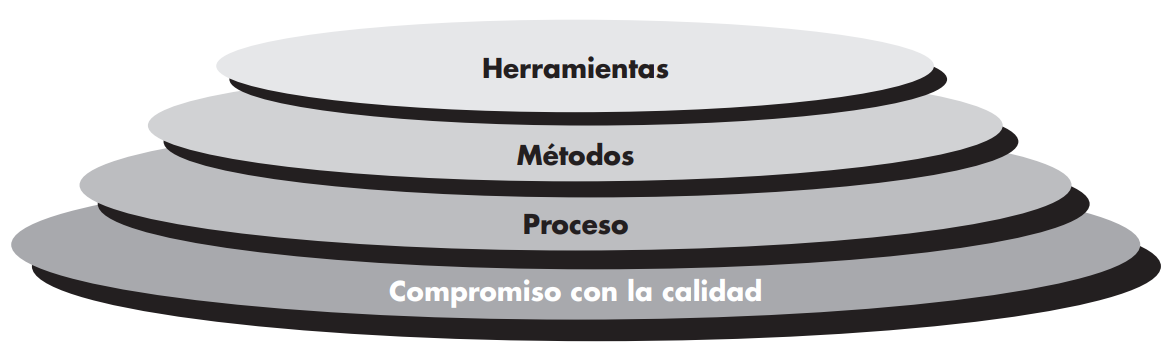
\includegraphics[width=.95\textwidth]{images/CapasIS}
		\caption{Pressman, R. (2010) Capas de la ingeniería de software.}
		\hyperlink{b09}{[9]}
		\label{fig:capas_is}
	\end{center}
\end{figure}

El proceso de software forma la base para el control de la administración de proyectos de software, y establece el contexto en el que se aplican métodos técnicos, se generan productos del trabajo (modelos, documentos, datos, reportes, formatos, etc.), se establecen puntos de referencia, se asegura la calidad y se administra el cambio de manera apropiada.\hyperlink{b09}{[9]} 

\newpage

\section{Proceso de desarrollo de software}

Hacer ingeniería de software implica realizar tareas para resolver problemas con base en un conjunto de principios fundamentales, para Pressman, la capa más importante y fundamental es la de Proceso, aquá se define el ``cascarón" del producto que se desea desarrollar.\\

Pressman define el proceso del software como: \\

``Una estructura para las actividades, acciones y tareas que se requieren a fin de construir software de alta calidad. La ingeniería de software es llevada a cabo por personas creativas y preparadas que deben adaptar un proceso maduro de software a fin de que resulte apropiado para los productos que construyen y para las demandas de su mercado.
Cuando se trabaja en la construcción de un producto o sistema, es importante ejecutar una serie de pasos predecibles, una estructura general para la ingeniería de software se define en cinco actividades elementales  \hyperlink{b09}{[9]}:"

\begin{enumerate}
	\item Comunicación
	\item Planeación
	\item Modelado
	\item Construcción
	\item Despliegue
\end{enumerate}

Existen diferentes metodologías de desarrollo con modificaciones y adecuaciones al esquema general de construcción antes mencionado, algunas de ellas son las metodologías tradicionales y ágiles. Este proceso puede tener diferentes variaciones, sin embargo, sea cual sea la metodología aplicada, las etapas de Modelado (Análisis y Diseño) y Costrucción (Codificación y Pruebas) son las más críticas e importantes para un producto final exitoso.\\

Durante el desarrollo, se realizan tareas específicas para cada etapa, por ejemplo, para la etapa de modelado se elabora el documento de análisis (donde se describe el funcionamiento del sistema), así como el diseño (en donde se genrean los diagramas que describen el funcionamiento establecido en el análisis); en la fase de construcción se genera el código del software y en la etapa de pruebas se valida y verifica que el software cumpla con lo asentado en las fases precedentes.

\subsection{Análisis}

``El proceso de análisis dentro del desarrollo de software consiste en obtener los requerimientos del sistema para crear una solución, identificar los problemas a resolver o necesidad a ser atendida, evaluar las restricciones que presenta, así como los insumos se requieren para su debida construcción.
Al ser la primera etapa dentro del proceso de desarrollo es las más crítica y sensible, ya que cualquier error de gran impacto que surja dentro de esta perjudicará las etapas consecuentes ocasionando retrasos en el proceso." \hyperlink{b09}{[9]} 

\bigskip

``Durante esta etapa se construye el documento de análisis, en donde se obtienen y describen todas las necesidades y peticiones del cliente en forma de requerimientos. Con base en estos, el analista continua el proceso identificando en alto nivel que funcionalidades deberá poseer el sistema para cumplir los requerimientos. Una solución común para mapear cada funcionalidad es a través de CASOS DE USO. Este documento proporciona la descripción de la manera en la que se utilizará el sistema y emplea un lenguaje técnico especializado ya que busca ser comprendido por los diseñadores y programadores para su correcta construcción." \hyperlink{b42}{[42]}


\subsubsection{Documento de análisis}

Con base en los enunciados del libro Ingeniería de Software, un enfoque práctico y la experiencia adquirida en el desarrollo de sistemas de la Coordinación de Desarrollo Tecnológico de la ESCOM, se propone la siguiente estructura para la construcción del documento de análisis.\\

Parte 1. Modelo de negocio:
\begin{itemize}
	\item Glosario de términos.
	\item Modelo de información utilizado para representar la información que será almacenada en el sistema.
	\item Reglas de negocio mediante las cuales se normará el funcionamiento del sistema.
\end{itemize}

Parte 2. Modelo dinámico, el cual describe funcionalidad a partir de los siguientes capítulos:
\begin{itemize}
	\item Arquitectura lógica.
	\item Máquinas de estados que modelarán el comportamiento de las entidades que así lo necesiten.
	\item Funciones y roles que tendrán los actores que interactuarán con el sistema.
	\item Casos de uso que describen funcionalidad.
\end{itemize}

Parte 3. Interacción con el usuario, que muestra las interfaces y mensajes a partir de los siguientes capítulos:
\begin{itemize}
	\item Interfaces del sistema.
	\item Catálogo de mensajes.
\end{itemize}


\subsubsection{Caso de Uso}

En un libro que analiza cómo escribir casos de uso eficaces, Alistair Cockburn afirma que: \textit { “un caso de uso capta un contrato que describe el comportamiento del sistema en distintas condiciones en las que el sistema responde a una petición de alguno de sus participantes."} \hyperlink{b43}{[43]}\\

Pressman toma esta definición como fundamento y la complementa proponiendo que un caso de uso es una actividad que puede realizar un usuario dentro del software y que sirven para describir el funcionamiento de los componentes acorde a las acciones que los usuarios realizan dentro del software, asegurando que:\\

\textit {``En esencia, un caso de uso narra una historia estilizada sobre cómo interactúa un usuario final (que tiene cierto número de roles posibles) con el sistema en circunstancias específicas. La historia puede ser un texto narrativo, un lineamiento de tareas o interacciones, una descripción basada en un formato o una representación diagramática. Sin importar su forma, un caso de uso ilustra el software o sistema desde el punto de vista del usuario final."} \hyperlink{b09}{[09]}\\

Para escribir casos de uso eficientes, el autor Alistair Cockburn presenta la esructura un Caso de uso básico que describe la interacción entre el actor y el sistema. Menciona que dependiendo de los requisitos podría haber casos de uso más detallados. 

Por ejemplo si se requiere hacer una descripción detallada del caso de uso sugiere el siguiente formato \hyperlink{b43}{[43]}: 

\begin{itemize}
\item \textbf{Nombre del caso de uso}
\item \textbf{Actor principal}
\item \textbf{Objetivo en contexto} 
\item \textbf{Disparador} 
\item \textbf{Escenario} 
\end{itemize}

Con base en los enunciados de Alistair Cockburn en su libro ``Escribiendo Casos de Uso efectivos" (2001) y en la experiencia en el análisis y desarrollo de sistemas de la Coordinación de Desarrollo Técnologico CDT, se propone la siguiente estructura para la presentación de un Caso de Uso, así como los elementos que lo componen y forman parte del caso de uso.

\begin{itemize}
\item \textbf{Actor}: Es la idealización de un rol que puede jugar una persona, otro sistema, proceso, un dispositivo o de alguna cosa que interactúa con el sistema. Los actores son objetos que residen fuera del sistema, en tanto que los casos de uso están compuestos por objetos y acciones que residen dentro del sistema. Todo actor tiene uno o más objetivos cuando utiliza el sistema.  \hyperlink{b12}{[12]}. 

\item \textbf{Entidad} : Representación de un objeto exclusivo único en el mundo real que se está controlando. Algunos ejemplos de entidad son una sola persona, un solo producto o una sola organización. \hyperlink{b44}{[44]}.

\item \textbf{Atributo} : Es una especificación que define una propiedad de un objeto, elemento o archivo. También puede referirse o establecer el valor específico para una instancia determinada de los mismos. \hyperlink{b44}{[44]}.

\item \textbf{Entrada}: Es la información producida por el usuario para ser guardada o procesada en el sistema. El usuario comunica y determina qué clases de entrada aceptará el sistema (por ejemplo, secuencias de control o de texto escritas a máquina a través del teclado y el ratón). \hyperlink{b45}{[45]}.

\item \textbf{Salida}: Es la información producida por el sistema y percibida por el usuario. Las clases de salida los productos de programa, y las clases de entrada la que el programa acepta, definen la interfaz de usuario del programa. \hyperlink{b45}{[45]}.

\item \textbf{Acción}: Evento originado por el usuario mediante botones.

\item \textbf{Pantalla}: Es la interfaz de usuario, utiliza imágenes, iconos y menús para mostrar las acciones disponibles entre las que el usuario puede escoger en un sistema. Su función es proporcionar un entorno visual amigable y sencillo de usar que facilite la comunicación del usuario con el software.\hyperlink{b46}{[46]}

\item \textbf{Regla de Negocio}: Es aquella que rige los procesos de un negocio para garantizar el correcto funcionamiento del software. Las reglas de negocio establecen los procedimientos que se deben realizar y las condiciones sobre las que dichas actividades se van a ejecutar.

\item \textbf{Mensaje}: Constituyen la mínima unidad de comunicación entre el usuario y el sistema. Se trata de un proceso de comunicación completa porque el sistema lanza un mensaje hacia el usuario que no se resuelve hasta que el usuario lo recibe o lo responde, completando así el proceso de comunicación con la realimentación correspondiente. \hyperlink{b47}{[47]}

\item \textbf{Trayectoria}: Es un conjunto de pasos que describen la interaccion entre el usuario y el sistema.

\item \textbf{Paso}: Es una instruccion que realiza el usuario o el sistema.

\item \textbf{Precondición}: Está formada por el conjunto de condiciones que se tienen que cumplir para que se pueda iniciar un caso de uso. En muchos casos supone la ejecución de casos de uso previos. \hyperlink{b48}{[48]}

\item \textbf{Postcondición}: Refleja el estado en que se queda el sistema una vez ejecutado el caso de uso. \hyperlink{b48}{[48]}

\item \textbf{Puntos de extensión}: Es la incorporación implícita del comportamiento de otro caso de uso, el cuál no es parte del flujo principal. Modela la parte opcional del sistema, un subflujo que sólo se ejecuta bajo ciertas condiciones o varios flujos que se pueden insertar en un punto determinado. \hyperlink{b49}{[49]}
\end{itemize}

A continuación se ilustra la estructura de la descripción de un caso de uso con todos sus elementos. En primera instancia se identifica el caso de uso con una clave y un nombre. Posteriormente, se redacta el resumen del caso de uso en un texto breve y conciso, tal como se muestra en el ejemplo de la Figura \ref{fig:resu}.

\begin{figure}[H]
	\begin{center}
		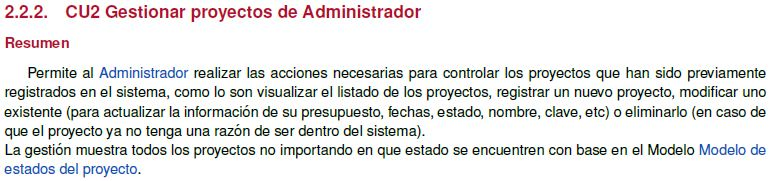
\includegraphics[width=1\textwidth]{images/marcoteorico/resumen}
		\caption{Ejemplo de identificador y resúmen de un caso de uso}
		\label{fig:resu}
	\end{center}
\end{figure}

Una vez redactado el resúmen del caso de uso se enlistan los atributos participes en esta descripción. Se especifica el rol del actor que interactua con el sistema, el propósito del caso de uso, entradas, salidas, precondiciones, postcondiciones, errores y tipo de caso de uso. En la Figura \ref{fig:atri} se muestra un ejemplo.

\begin{figure}[H]
	\begin{center}
		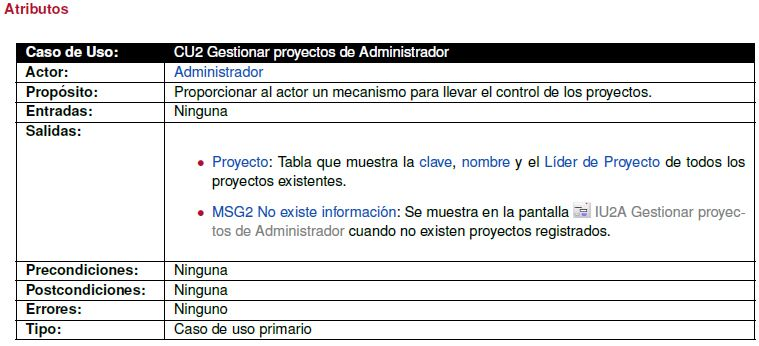
\includegraphics[width=1\textwidth]{images/marcoteorico/atributos}
		\caption{Ejemplo de la descripción de atributos del caso de uso}
		\label{fig:atri}
	\end{center}
\end{figure}

Posteriormente se realiza la descripción de trayectorias con sus pasos, la primera es la trayectoria principal y es aquella que se sigue el flujo normal del caso de uso. También están las alternativas que como su nombre lo dice flujos alternativos que están contemplados pero no forman parte del proceso principal.\\

En la redacción de los pasos se hace referencia a las pantallas, mensajes, reglas de negocio y otras trayectorias que se ven involucrados en la interacción del actor con el sistema.
Un ejemplo se muestra en la Figura \ref{fig:trayectoriap}

\begin{figure}[H]
	\begin{center}
		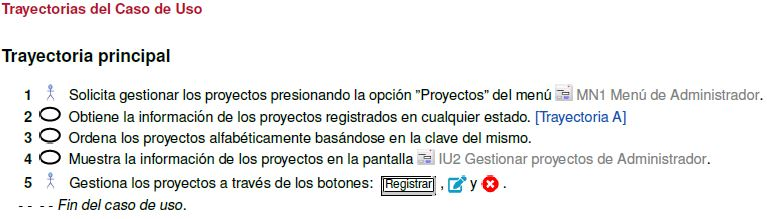
\includegraphics[width=1\textwidth]{images/marcoteorico/trayectorias}
	\end{center}
\end{figure}

\begin{figure}[H]
	\begin{center}
		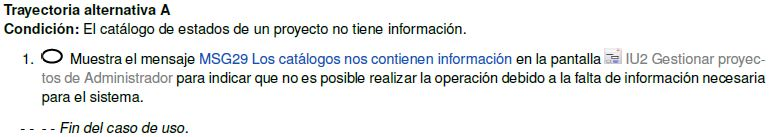
\includegraphics[width=1\textwidth]{images/marcoteorico/alternativa}
		\caption{Ejemplo de la descripción de trayectorias del caso de uso}
		\label{fig:trayectoriap}
	\end{center}
\end{figure}

\newpage

Finalmente, en la especificación se describen los puntos de extensión del caso de uso tal como se muestra en la Figura \ref{fig:puntos}

\begin{figure}[H]
	\begin{center}
		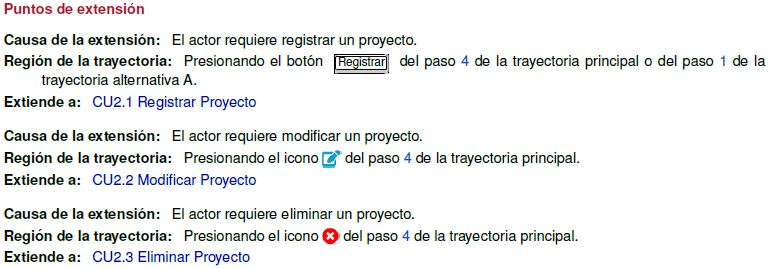
\includegraphics[width=1\textwidth]{images/marcoteorico/puntosdeextension}
		\caption{Ejemplo de la descripción de trayectorias del caso de uso}
		\label{fig:puntos}
	\end{center}
\end{figure}

\newpage

\section{Herramienta CASE}

\subsection{Definición}

Las tecnologías de ingeniería de software asistida por computadora (Computer Aided Software Engineering, CASE por sus siglas en inglés), \textit {``son herramientas que brindan asistencia automatizada para el desarrollo de software. El objetivo de presentar las herramientas CASE es la reducción del tiempo y el costo del desarrollo de software y la mejora de la calidad de los sistemas desarrollados."} \hyperlink{b15}{[15]}\\

El interés en las herramientas y entornos de CASE se basa en las expectativas de: \hyperlink{b15}{[15]}
\begin{itemize}
	\item Aumentar la productividad
	\item Mejorar la calidad del producto
	\item Facilitar el mantenimiento
	\item Hacer que la tarea de los ingenieros de software sea menos tediosa y más agradable. 
\end{itemize}

Una herramienta CASE se puede clasificar en tres categorías: \hyperlink{b50}{[50]}

\begin{itemize}
	\item Upper CASE (U-CASE), herramientas que ayudan en las fases de planificación, análisis de requisitos y estrategia del desarrollo, usando, entre otros diagramas UML.
	\item Middle CASE (M-CASE), herramientas para automatizar tareas en el análisis y diseño de la aplicación.
	\item Lower CASE (L-CASE), herramientas que semi-automatizan la generación de código, crean programas de detección de errores, soportan la depuración de programas y pruebas. Además automatizan la documentación completa de la aplicación. Aquí pueden incluirse las herramientas de desarrollo rápido de aplicaciones.
\end{itemize}

Debido a sus similitudes, a veces Upper CASE y Middle CASE simplemente se conocen como Upper CASE. En general, Upper CASE es una herramienta para una vista de alto nivel del desarrollo de software, mientras que lower CASE se utiliza principalmente como herramienta en la fase de programación y prueba. \hyperlink{b16}{[16]}

\newpage

\section {Implementación del desarrollo}

\subsection{Patrones de diseño}

Cada patrón describe un problema que ocurre una y otra vez en nuestro entorno, también describe el núcleo de la solución a ese problema, de tal manera que puede usar esta solución un millón de veces, sin tener que hacerlo lo mismo dos veces. \hyperlink{b19}{[19]} \\

En general, un patrón tiene cuatro elementos esenciales \hyperlink{b17}{[17]}:

\begin{enumerate}
	\item ``El nombre del patrón es un identificador que podemos usar para describir un problema de diseño, sus soluciones y consecuencias en una o dos palabras. Nombrar un patrón nos permite diseñar a un nivel más alto de abstracción."
	
	\item ``El problema describe cuándo aplicar el patrón. Explica el problema y su contexto. Podría describir problemas de diseño específicos, como la forma de representar algoritmos como objetos. Podría describir estructuras de clase u objeto que son sintomáticas de un diseño inflexible. A veces, el problema incluirá una lista de condiciones que deben cumplirse antes de que tenga sentido aplicar el patrón."
	
	\item ``La solución describe los elementos que componen el diseño, sus relaciones, responsabilidades y colaboraciones. La solución no describe un diseño o implementación concreta en particular, porque un patrón es como una plantilla que se puede aplicar en muchas situaciones diferentes. En cambio, el patrón proporciona una descripción abstracta de un problema de diseño y cómo lo resuelve una disposición general de elementos (clases y objetos en nuestro caso)."
	
	\item ``Las consecuencias son los resultados y las compensaciones de aplicar el patrón. Aunque las consecuencias a menudo no se expresan cuando describimos las decisiones de diseño, son críticas para evaluar las alternativas de diseño y para comprender los costos y beneficios de aplicar el patrón. Las consecuencias para el software a menudo se refieren a compensaciones de espacio y tiempo. También pueden abordar problemas de lenguaje e implementación. Dado que la reutilización es a menudo un factor en el diseño orientado a objetos, las consecuencias de un patrón incluyen su impacto en la flexibilidad de un sistema, extensibilidad o portabilidad. Enumerar estas consecuencias explícitamente le ayuda a comprenderlas y evaluarlas."
\end{enumerate}

\subsubsection{Patrón de Diseño MVC (Modelo Vista-Controlador)}

El patrón de diseño de Modelo-Vista-Controlador (Model–View–Controller, MVC por sus siglas en inglés) especifica que una aplicación consta de un modelo de datos, de información de presentación y de información de control. El patrón requiere que cada uno de estos elementos esté separado en distintos objetos. \hyperlink{b18}{[18]}

\subsubsection{Características}
MVC consta de tres tipos de objetos \hyperlink{b18}{[18]}: 
\begin{enumerate}
\item ``El modelo es el objeto de la aplicación (por ejemplo, la información de datos) contiene únicamente los datos puros de aplicación; no contiene lógica que describe cómo pueden presentarse los datos a un usuario."
\item ``La vista es su presentación en pantalla  (por ejemplo, la información de presentación) presenta al usuario los datos del modelo. La vista sabe cómo acceder a los datos del modelo, pero no sabe el significado de estos datos ni lo que el usuario puede hacer para manipularlos."
\item ``Por último, el controlador que  define la forma en que la interfaz de usuario reacciona a la entrada del usuario(por ejemplo, la información de control) está entre la vista y el modelo. Escucha los sucesos desencadenados por la vista (u otro origen externo) y ejecuta la reacción apropiada a estos sucesos. En la mayoría de los casos, la reacción es llamar a un método del modelo. Puesto que la vista y el modelo están conectados a través de un mecanismo de notificación, el resultado de esta acción se reflejará automáticamente en la vista."
\end{enumerate}

El comportamiento y comunicación de este modelo se ilustra en la Figura \ref{fig:mvc}

\begin{figure}[H]
	\begin{center}
		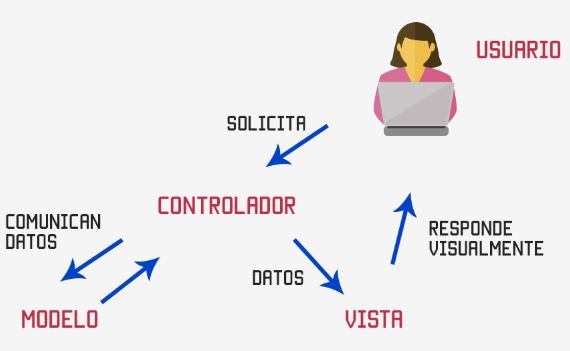
\includegraphics[width=.75\textwidth]{images/marcoteorico/mvc}
		\caption{Peress, H. (2015) Código Facilito: Ilustración del Modelo Vista Controlador.}
		\hyperlink{b51}{[51]} 
		\label{fig:mvc}
	\end{center}
\end{figure}

\newpage

MVC desacopla las vistas y los modelos al establecer un protocolo de suscripción / notificación entre ellos. Una vista debe garantizar que su apariencia refleje el estado del modelo. Cada vez que los datos del modelo cambian, el modelo notifica las vistas que dependen de él. En respuesta, cada vista tiene la oportunidad de actualizarse. Este enfoque le permite adjuntar múltiples vistas a un modelo para proporcionar diferentes presentaciones. También puede crear nuevas vistas para un modelo sin reescribirlo.\\

En la Figura \ref{fig:mvc2} se muestra un modelo y tres vistas. (Se omitieron los controladores por simplicidad). El modelo contiene algunos valores de datos, y las vistas que definen una hoja de cálculo, un histograma y un gráfico circular muestran estos datos de varias maneras. El modelo se comunica con sus vistas cuando cambian sus valores, y las vistas se comunican con el modelo para acceder a estos valores. \hyperlink{b20}{[20]} 

\begin{figure}[H]
	\begin{center}
		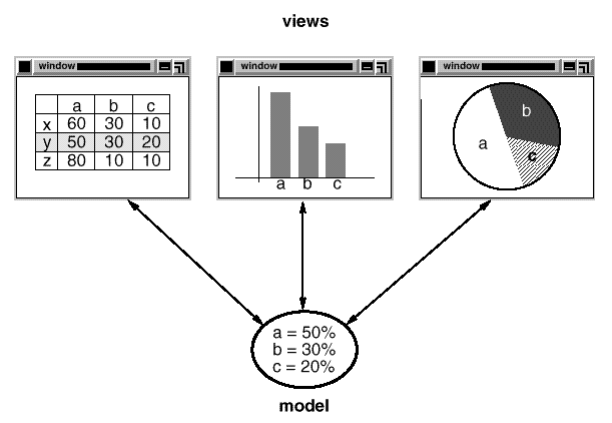
\includegraphics[width=.85\textwidth]{images/marcoteorico/mvc2}
		\caption{Glenn E. Krasner (1988) Ejemplo práctico de cómo opera el MVC}
		\hyperlink{b20}{[20]} 
		\label{fig:mvc2}
	\end{center}
\end{figure}

\newpage

\subsubsection{Singleton}
Es un patrón diseñado para limitar la creación de objetos pertenecientes a una clase. El objetivo de este patrón es el de garantizar que una clase solo tenga una instancia (o ejemplar) y proporcionar un punto de acceso global a ella. Suele ser utilizado para las conexiones a bases de datos, se implementa haciendo privado el constructor de la clase y creando (en la propia clase) un método que crea una instancia del objeto si este no existe. \hyperlink{b70}{[70]}\\

El patrón utiliza variables y métodos de clase estáticos para la implementación global y la unicidad de la instanciación de la clase. La Figura \ref{fig:single} muestra esta estructura simple pero poderosa.\\

\begin{figure}[H]
	\begin{center}
		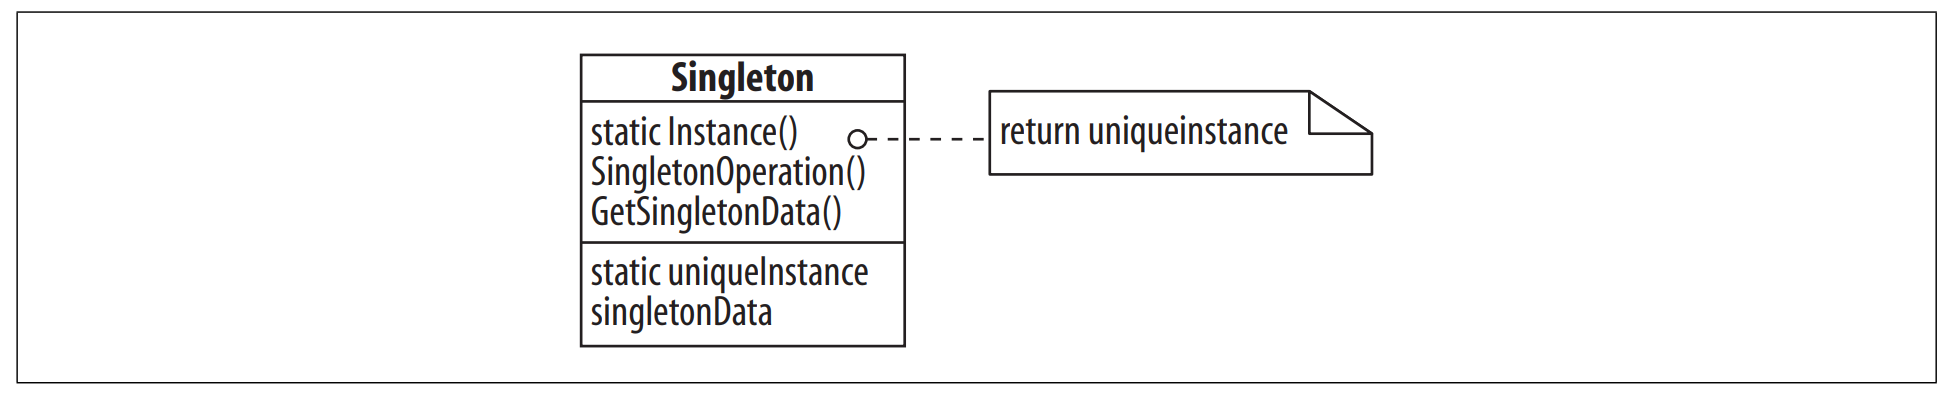
\includegraphics[width=1\textwidth]{images/marcoteorico/patrones/singleton}
		\caption{ Sanders, W. B. Y Cumaranatunge, C. (2007) Estructura Singleton}
		\hyperlink{b72}{[72]} 
		\label{fig:single}
	\end{center}
\end{figure}

\subsubsection{Factory}
Factory Method permite la creación de objetos de un subtipo determinado a través de una clase Factory. Esto es especialmente útil cuando no sabemos, en tiempo de diseño, el subtipo que vamos a utilizar o cuando queremos delegar la lógica de creación de los objetos a una clase Factory. Utilizando este patrón podemos crear instancias dinámicamente mediante la configuración, estableciendo cual será la implementación a utilizar en un archivo de texto de Lenguaje de Marcado Extensible (Extensible Markup Language, XML por sus siglas en inglés) properties o mediante cualquier otra estrategia. \hyperlink{b70}{[70]}\\

La Figura \ref{fig:factory} muestra el modelo de alto nivel del patrón. Varios clientes pueden usar el método factory en un creator para acceder y usar múltiples products. La naturaleza intermediaria del creator es clara en este modelo, ya que obliga a la creación de múltiples tipos de objetos (diferentes productos) a través de un punto común. \hyperlink{b72}{[72]} 

\begin{figure}[H]
	\begin{center}
		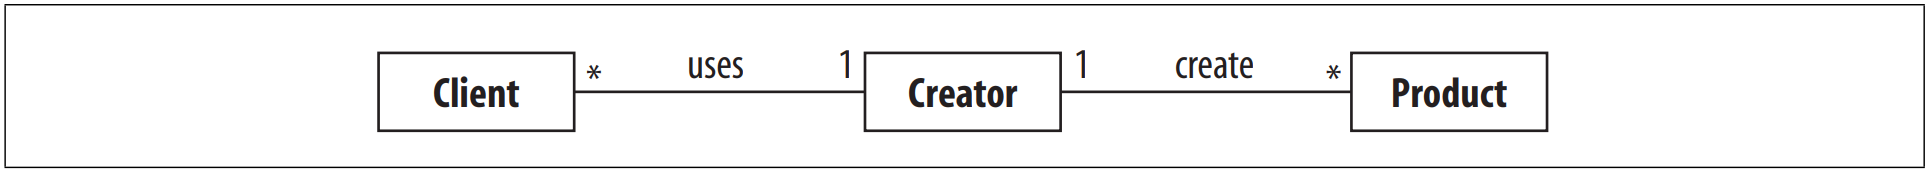
\includegraphics[width=1\textwidth]{images/marcoteorico/patrones/factory}
		\caption{ Sanders, W. B. Y Cumaranatunge, C. (2007) Modelo Lógico del Patrón Factory}
		\hyperlink{b72}{[72]} 
		\label{fig:factory}
	\end{center}
\end{figure}

Una de las principales ventajas del patrón de método factory es la extensibilidad que ofrece para adaptarse al cambio \hyperlink{b72}{[72]}. Veamos el diagrama de clases del patrón en la Figura \ref{fig:factory2} .

\begin{figure}[H]
	\begin{center}
		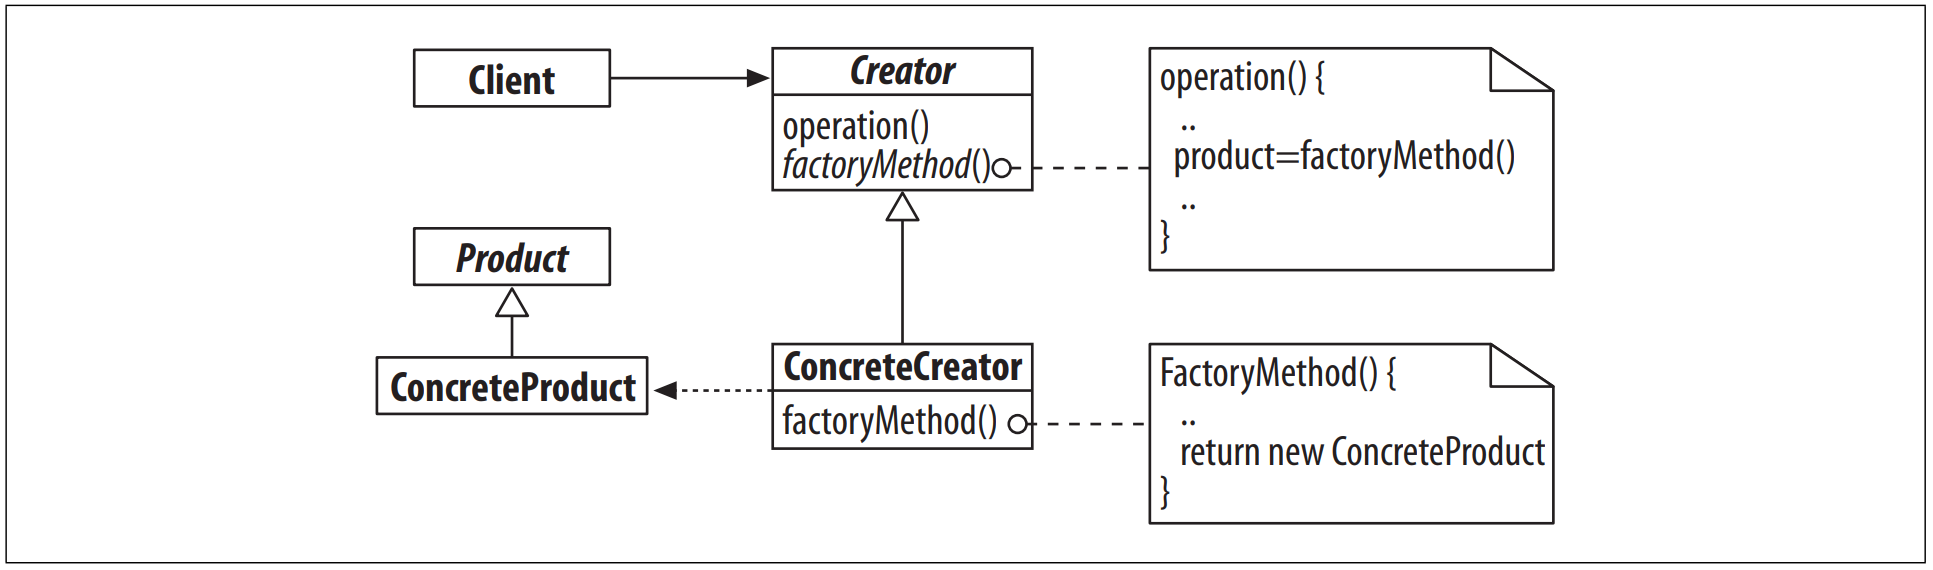
\includegraphics[width=1\textwidth]{images/marcoteorico/patrones/factory2}
		\caption{ Sanders, W. B. Y Cumaranatunge, C. (2007) Diagrama de Clases del Patrón Factory}
		\hyperlink{b72}{[72]} 
		\label{fig:factory2}
	\end{center}
\end{figure}

\subsubsection{Facade (Fachada)}
El patrón Facade (fachada) tiene la característica de ocultar la complejidad de interactuar con un conjunto de subsistemas proporcionando una interface de alto nivel, la cual se encarga de realizar la comunicación con todos los subsistemas necesarios. La fachada es una buena estrategia cuando requerimos interactuar con varios subsistemas para realizar una operación concreta ya que se necesita tener el conocimiento técnico y funcional para saber qué operaciones de cada subsistema tenemos que ejecutar y en qué orden, lo que puede resultar muy complicado cuando los sistemas empiezan a crecer demasiado. \hyperlink{b70}{[70]}

\subsubsection{Adapter (Adaptador)}
El patrón adaptador se utiliza para transformar una interfaz en otra, de tal modo que una clase que no pueda utilizar la primera haga uso de ella a través de la segunda. Convierte la interfaz de una clase en otra interfaz que el cliente espera. El adaptador permite a las clases trabajar juntas, lo que de otra manera no podría hacerse debido a sus interfaces incompatibles. \hyperlink{b70}{[70]}\\

Todas las clases de adaptadores implementan una interfaz. En el diagrama de clases que se muestra en la Figura \ref{fig:adapter} , la interfaz llamada ITarget declara un método único llamado request (). El diagrama de clase muestra que una referencia a una instancia de la clase Adaptee se almacena en la variable adaptee. Al implementar el método request (), el adaptador hace referencia a esta instancia. \hyperlink{b72}{[72]}

\begin{figure}[H]
	\begin{center}
		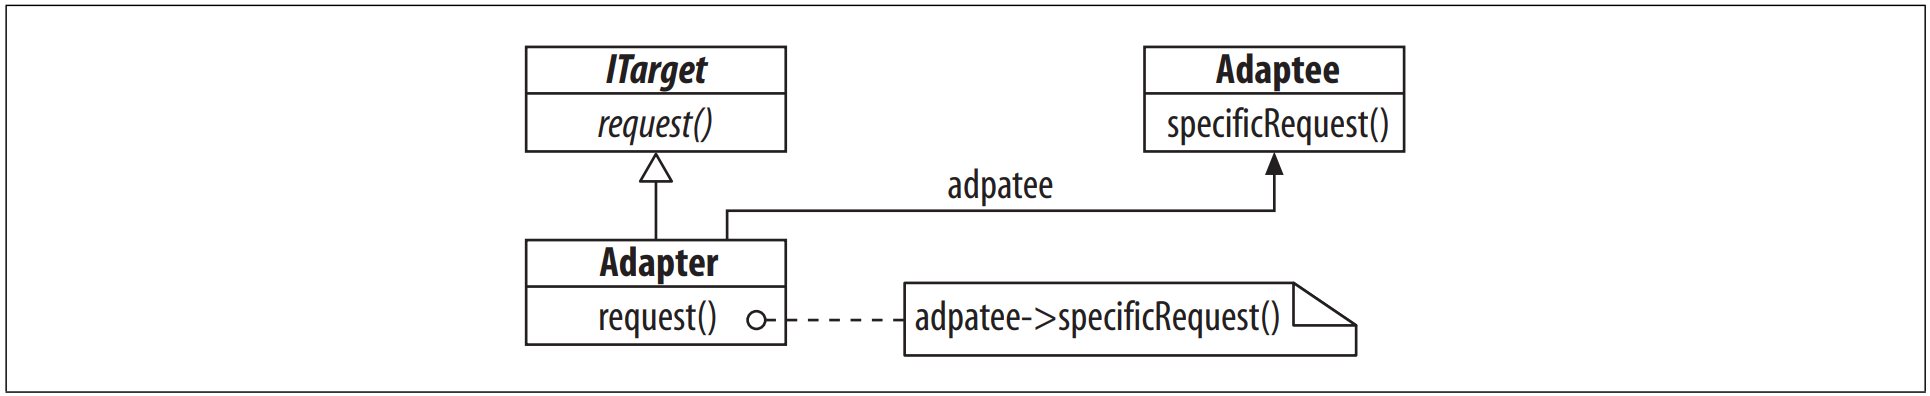
\includegraphics[width=1\textwidth]{images/marcoteorico/patrones/adapter}
		\caption{ Sanders, W. B. Y Cumaranatunge, C. (2007) Diagrama de Clases de un Objeto Adapter}
		\hyperlink{b72}{[72]} 
		\label{fig:adapter}
	\end{center}
\end{figure}

\subsubsection{Data Access Object (DAO)}
La capa DAO contiene todos los métodos CRUD (create, read, update, delete), por lo general se tiene un DAO para cada tabla en la base de datos. \hyperlink{b71}{[71]}

\subsubsection{Data Transfer Object (DTO)}
Se utiliza para transferir varios atributos entre el cliente y el servidor o viceversa, básicamente consta de 2 clases:

La primera es una clase java conocida como Value Object que únicamente contiene sus atributos, constructor, getters y setters, esta clase no tiene comportamiento.
La segunda es una clase del lado del servidor conocida como clase de negocio (en la implementación también se conoce como Business Object) es la que se encarga de obtener datos desde la base de datos y llenar la clase Value Object y enviarla al cliente, o a su vez recibir la clase desde el cliente y enviar los datos al servidor, por lo general tiene todos los métodos CRUD (create, read, update y delete). \hyperlink{b71}{[71]}

\subsubsection{Decorator}
El patrón Decorator en Java permite agregar nuevas funcionalidades a las clases sin modificar su estructura.
El concepto de este patrón es agregar de forma dinámica nuevo comportamiento o funcionalidades a la clase principal.
La definición oficial dice que “permite el ajuste dinámico de objetos para modificar sus responsabilidades y comportamientos existentes.”  \hyperlink{b71}{[71]}

En la Figura \ref{fig:decorator} de ilustra el diagrama de clase del Patrón Decorator.

 \begin{figure}[H]
 	\begin{center}
 		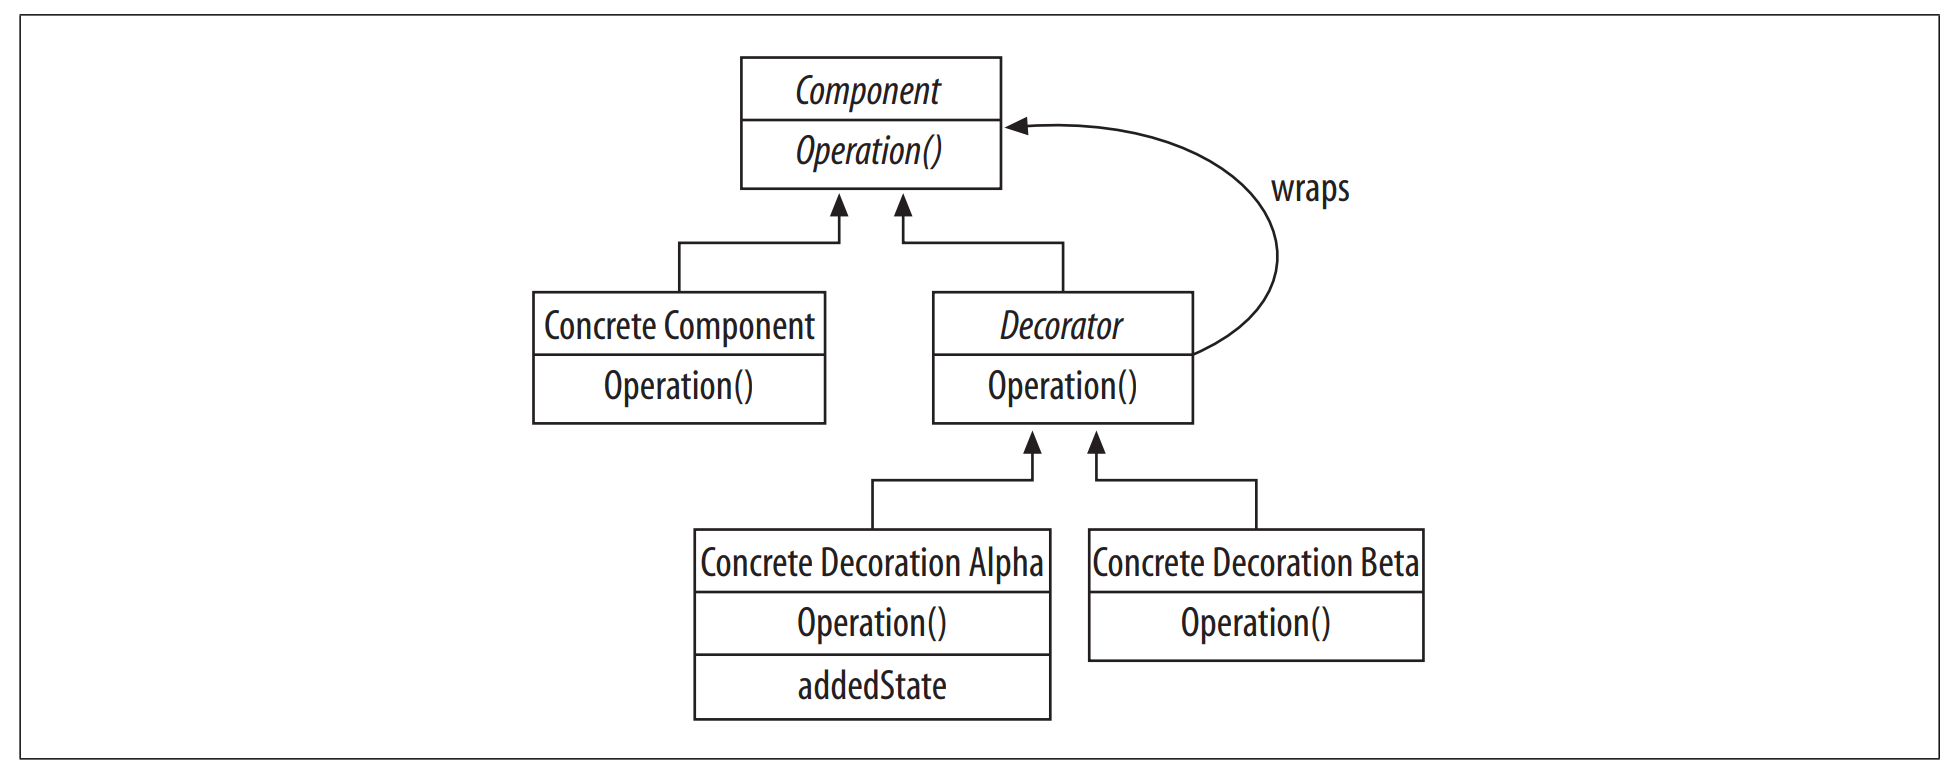
\includegraphics[width=1\textwidth]{images/marcoteorico/patrones/decorator}
 		\caption{ Sanders, W. B. Y Cumaranatunge, C. (2007) Patrón de Diseño Decorator}
 		\hyperlink{b72}{[72]} 
 		\label{fig:decorator}
 	\end{center}
 \end{figure}


\subsection{Framework}

\subsubsection{Definición}

Erich Gamma en su libro "Patrones de diseño: Elementos de software orientado a objetos reutilizables" define un framework como:\\ 

\textit {``Un conjunto de clases cooperativas que construyen un diseño reutilizable para un tipo específico de software. Un Framework proporciona la arquitectura partiendo el diseño en clases abstractas y definiendo sus responsabilidades y colaboraciones. Un desarrollador realiza una aplicación haciendo subclases y componiendo instancias a partir de las clases definidas por el Framework."} \hyperlink{b17}{[17]}. \\

Un framework es una aplicación semi-completa, de control invertido, así un Framework difiere de una librería de clases \hyperlink{b17}{[17]}: 
\begin{itemize}
	\item ``En una librería de clases, el control del flujo se encuentra en el código de la aplicación que realiza llamadas a los métodos de la librería de clases."
	\item ``En un framework, el control del flujo está en código del framework que realiza llamadas al código de la aplicación (control invertido)."
\end{itemize}
\subsubsection {Ventajas de un framework}
Como ventajas en la utilización de un framework tenemos las siguientes \hyperlink{b52}{[52]}: 

\begin{enumerate}
	\item ``Minimiza tiempos de desarrollo"
	\begin{itemize}
	\item ``Los proyectos de desarrollo ya no tendrán que resolver los múltiples problemas asociados a las aplicaciones Web."
	\item ``Los frameworks reducen la codificación y sobretodo la puesta en marcha, ya que proporcionan subsistemas que sabemos que ya funcionan."
	\item ``Proporcionan código que no se tendrá que mantener ni reescribir."
	\end{itemize}
	\item ``Reduce los riesgos del desarrollo."
	\begin{itemize}
		\item Con un modelo de programación complejo como el de la Plataforma de Java Edición Empresarial (Java Platform Enterprise Edition, Java EE por sus siglas en inglés), el riesgo de fallos en los proyectos iniciales es alto.
	\end{itemize}
	\item ``Proporciona una arquitectura consistente entre aplicaciones."
	\begin{itemize}
		\item Al usar frameworks todas las aplicaciones generadas comparten una arquitectura común. Esto hace que sea más fácil de aprender, mantener y soportar.
		\item Cualquier programador que trabaje con un framework no deberá invertir gran parte de su tiempo en buscar las clases necesarias, interconectarlas o descubrir los métodos que contienen. Los frameworks ocultan toda esta complejidad dando un alto nivel de abstracción. 
	\end{itemize}
\end{enumerate}

\subsection {Spring}
Spring nos brinda ventajas como: la administración de objetos, garantizando que los recursos se creen, reutilicen y limpien correctamente (Managed Objects) \hyperlink{b25}{[25]}; El Manejo de transacciones declarativas, por ejemplo Rollback de una transacción \hyperlink{b26}{[26]} y un modelo de programación consistente en diferentes interfaces de programación de aplicaciones (Application Programming Interface, API por sus siglas en inglés) de transacciones, tal como Java Persistence API.

\subsection {Struts}
Se implementó Struts2 porque es un framework de código abierto, extensible mediante plugins ( Transferencia de estado representacional (representational state transfer, REST por sus siglas en inglés), Asíncrono de Javascript y XML (Asynchronous JavaScript And XML, AJAX por sus siglas en inglés), etc) y utiliza el patrón de diseño MVC. \hyperlink{b27}{[27]} \\ 

Las ventajas ofrecidas por este framework son: 

\begin{itemize}
	\item Patron Observador (Observer pattern), las vistas se actualizan por sí mismas del modelo. \hyperlink{b28}{[28]}
	\item Provee un bajo acoplamiento entre la vista y el modelo haciendo aplicaciones significativamente más fáciles de crear y mantener. \hyperlink{b28}{[28]}
	\item Uso de Interceptores, ejecutan código antes y después de que un Action es invocado, por ejemplo al subir un archivo .\hyperlink{b29}{[29]}
\end{itemize}


\section{Pruebas}

Con base en los enunciados del Comité Internacional de Certificaciones de Pruebas de Softwarela (International Software Testing Qualifications Board, ISTQB por sus siglas en inglés). Las pruebas de software muestran la presencia de defectos:\\

 \textit {``Todo tipo de software que se desarrolle es susceptible a la presencia de «Bug`s» o defectos y con las pruebas de software se busca reducir al máximo la presencia de estos".} \hyperlink{b34}{[34]} \\

También no dice que existen diferentes técnicas de prueba de software, cada una con sus propias ventajas y desventajas. Cada uno de las técnicas es buena para encontrar ciertos tipos  de defectos y mala para detectar otros tipos, por lo cual se complementa una con otra.\\

En resumen, existen dos categorías principales, estática y dinámica. Las cuales se ilustran en la Figura \ref{fig:tecnicas}
 
\begin{figure}[H]
	\begin{center}
		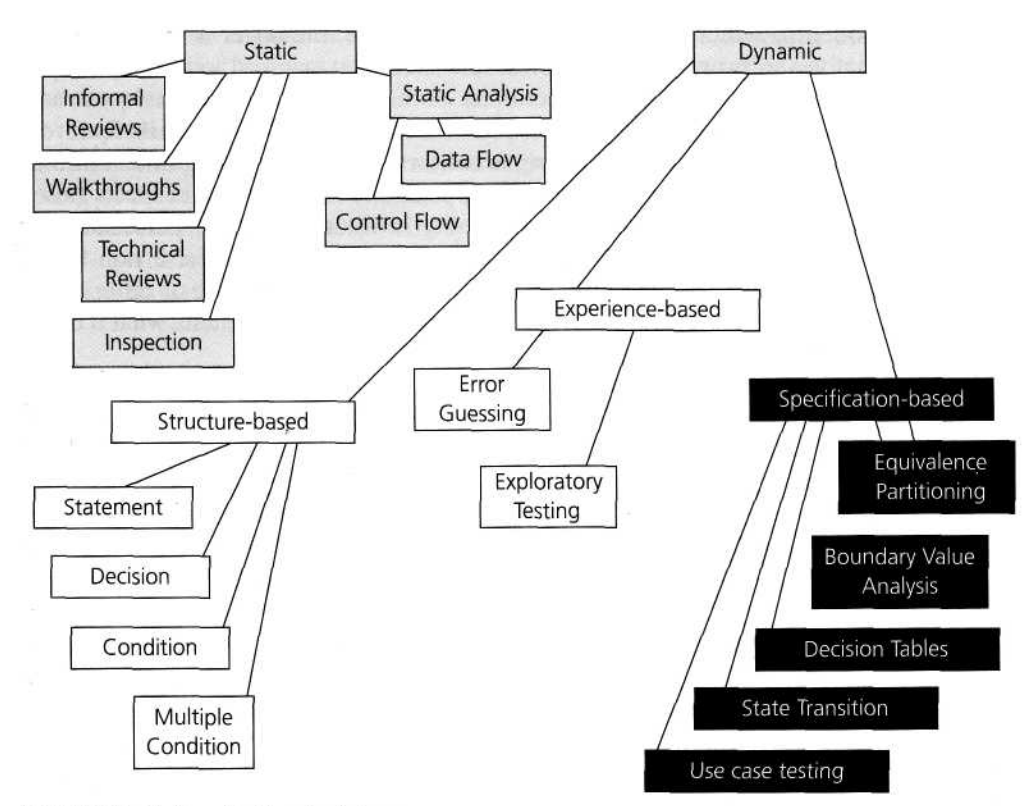
\includegraphics[width=.80\textwidth]{images/marcoteorico/tecnicas}
		\caption{ISTQB Foundations of Software Testing. Imagen que ilustra las técnicas de pruebas}
		\label{fig:tecnicas}
		\hyperlink{b34}{[34]}
	\end{center}
\end{figure}

\subsection{Pruebas Dinámicas}

La ISTQB (International Software Testing Qualifications Board) menciona que:

\textit {``Las pruebas dinámicas son todas aquellas pruebas que para su realización requieren la ejecución de la aplicación. Las pruebas dinámicas permiten el uso de técnicas de caja negra y caja blanca con mayor amplitud."} \hyperlink{b34}{[34]} 

A continuación se explica su utilidad \hyperlink{b34}{[34]}:  

\begin{enumerate}
	\item \textbf {Pruebas de caja negra o basadas en especificación}: ``Se conocen como técnicas de prueba impulsadas por entrada / salida porque ven el software como un recuadro negro con entradas y salidas, pero no se tiene un conocimiento de cómo se estructura el sistema o componente dentro de la caja. En esencia, está concentrando en lo que hace el software, no en cómo lo hace."
	
		La definición menciona pruebas tanto funcionales como no funcionales.
		\begin{itemize}
			\item \textbf {Pruebas Funcionales}: ``Se refieren a lo que hace el sistema, sus características o funciones".
			\item \textbf {Pruebas No Funcionales}: ``Se refieren a examinar qué tan bien el sistema hace algo, en lugar de lo que hace. Los aspectos no funcionales (también conocidos como características de calidad o atributos de calidad) incluyen rendimiento, usabilidad, portabilidad, mantenibilidad, etc."
		\end{itemize}
	
		Existen cinco técnicas basadas en especificaciones las cuales son \hyperlink{b34}{[34]}: 
		\begin{itemize}
			\item \textbf {Clases de equivalencia}: ``La idea detrás de la técnica es dividir un conjunto de condiciones de prueba en grupos o conjuntos que se pueden considerar iguales. La técnica requiere que solo necesitemos probar una condición de cada partición. Si una condición en una partición funciona o no, asumimos que todas las condiciones en esa partición tendrán el mismo comportamiento."
			\item \textbf {Análisis del valor límite}: ``Se basa en pruebas en los límites entre particiones. Opera realizado la 'verificación de rango', se tiene que tener en cuenta que tenemos límites válidos (en las particiones válidas) y límites inválidos (en las particiones inválidas)".
			\item \textbf {Tablas de decisión}: ``Proporcionan una forma sistemática de establecer reglas de negocios comerciales complejas. Ayudan a explorar los efectos de combinaciones de diferentes entradas y otros estados de software que deben implementar correctamente las reglas de negocio. Ayudan a la selección sistemática de casos de prueba efectivos, pueden encontrar problemas y ambigüedades en la especificación. Es una técnica que funciona bien junto con la partición de equivalencia. La combinación de condiciones exploradas puede ser combinaciones de particiones de equivalencia."
			\item \textbf {Prueba de transición de estado}: ``Se utiliza cuando se puede describir algún aspecto del sistema en lo que se llama una "máquina de estados finitos". Esto simplemente significa que el sistema puede estar en un número (finito) de estados diferentes, y las transiciones de un estado a otro están determinadas por las reglas de la 'máquina'."
			\item \textbf {Prueba de caso de uso}:
			``La prueba de casos de uso es una técnica que nos ayuda a identificar casos de prueba que ejercitan todo el sistema transacción por transacción de principio a fin. Ivar Jacobson los describe en su libro Ingeniería de software orientada a objetos: un enfoque orientado a casos de uso [Jacobson, 1992]."
		\end{itemize}
	
	\item \textbf {Pruebas de caja blanca}: ``Las técnicas de prueba basadas en la estructura utilizan la estructura interna del software para derivar casos de prueba. Se denominan comúnmente técnicas de 'caja blanca' o 'caja de cristal' (lo que implica que puede ver el sistema), ya que requieren conocer cómo se implementa el software, es decir, cómo funciona. Por ejemplo, una técnica estructural puede estar relacionada con el ejercicio de bucles en el software."
	
	\item \textbf {Basadas en experiencia}: ``En las técnicas basadas en la experiencia, el conocimiento, las habilidades y los antecedentes de las personas son los principales contribuyentes a las condiciones y casos de prueba. La experiencia de los técnicos y los empresarios aporta diferentes perspectivas al análisis de prueba y al proceso de diseño ya pueden tener información sobre lo que podría salir mal, lo cual es muy útil para las pruebas."

\end{enumerate}

Dentro de las pruebas dinámicas podemos encontrar distintos niveles de prueba, estas son tareas que se gestionan juntas. En cada nivel se puede encontrar una instancia del proceso de prueba.\\

Los niveles de prueba utilizados pueden ser \hyperlink{b35}{[35]}: 

\begin{itemize}
	\item \textbf {Prueba de Componente}
	\item \textbf {Prueba de Integración}
	\item \textbf {Prueba de Sistema}
	\item \textbf {Prueba de Aceptación}
\end{itemize}

Los niveles de prueba se caracterizan por los siguientes atributos \hyperlink{b35}{[35]}: 

\begin{itemize}
	\item \textbf {Objetivos específicos}
	\item \textbf {Base de prueba, referenciada para derivar casos de prueba}
	\item \textbf {Objeto de prueba (es decir, lo que se está probando)}
	\item \textbf {Defectos y fallas típicas}
\end{itemize}

\subsubsection{Prueba de sistema}

El ISTQB centra las pruebas de sistema en el funcionamiento y capacidades del software.\\

 	\textit {``Para este nivel se consideran las tareas de extremo a extremo que el sistema puede realizar y los comportamientos no funcionales que exhibe mientras realiza esas tareas. Este nivel de pruebas tiene como objetivo: la reducción de riesgos, verificar si los comportamientos funcionales y no funcionales del sistema son los diseñados y especificados, alidar que el sistema está completo y funcionará como se esperaba, generar confianza en la calidad del sistema en su conjunto, encontrar defectos y Evitar que los defectos escapen a niveles de prueba o producción más altos."}\hyperlink{b35}{[35]} \\
 	
 	En el Cuadro \ref{tbl:basesyobjetos},  se describe cuales son las bases de prueba y los objetos de prueba para el nivel de sistema.
 

\begin{table}[H]
	\centering
	\begin{tabular}{|p{3.5cm}|p{13cm}|}
		\hline
		\centering \textbf{Base de prueba} & \begin{itemize}
			\item Especificaciones de requisitos del sistema y software (funcionales y no funcionales)
			\item Informes de análisis de riesgos.
			\item Casos de uso
			\item Epicas e historias de usuarios.
			\item Modelos de comportamiento del sistema.
			\item Diagramas de estado.
			\item Sistema y manuales de usuario.
		\end{itemize}
		  \\
		\hline
		\centering \textbf{Objeto de prueba} & \begin{itemize}
			\item Aplicaciones (de escritorio o móviles)
			\item Sistemas de hardware / software
		\end{itemize}  \\
		\hline
	\end{tabular}
\caption{Cuadro que describe las bases y objetos de prueba para el nivel de pruebas de sistema.}
\label{tbl:basesyobjetos}
\hyperlink{b35}{[35]}
\end{table}


\subsection{Pruebas Estáticas}

El ISTQB afirma que:\\

\textit {``Las pruebas estáticas encuentran defectos en los productos de trabajo directamente en lugar de identificar fallas causadas por defectos cuando se ejecuta el software.  En comparación con las pruebas dinámicas, los defectos típicos que son más fáciles y baratos de encontrar y reparar mediante pruebas estáticas incluyen:"} \hyperlink{b34}{[34]}
\begin{itemize}
	\item \textbf {``Defectos de requisitos"} (inconsistencias, ambigüedades, contradicciones, omisiones, imprecisiones y redundancias)
	\item \textbf {``Defectos de diseño"} (algoritmos ineficientes o estructuras de bases de datos, alto acoplamiento, baja cohesión)
	\item \textbf {``Defectos de codificación"} (variables con valores indefinidos, variables que se declaran pero nunca se usan, código inalcanzable, código duplicado)
	\item \textbf {``Desviaciones de los estándares"} (falta de adherencia a los estándares de codificación)
\end{itemize}

La mayoría de los tipos de defectos de mantenimiento solo se pueden encontrar mediante pruebas estáticas (por ejemplo, modularización inadecuada, mala reutilización de componentes, código que es difícil de analizar y modificar sin introducir nuevos defectos).A diferencia de las pruebas dinámicas, las pruebas estáticas encuentran defectos en lugar de fallas. \hyperlink{b34}{[34]}\\

\subsubsection {Defectos de Codificación}

Para el análisis estático hay muchas herramientas, y la mayoría de ellas se centran en el código de software. Las herramientas pueden mostrar no solo atributos estructurales (métricas de código), como la profundidad de anidamiento o el número ciclomático y verificar los estándares de codificación, sino también representaciones gráficas del flujo de control, las relaciones de datos y el número de rutas distintas de una línea de código a otra. Incluso el compilador puede considerarse una herramienta de análisis estático, ya que crea una tabla de símbolos, señala el uso incorrecto y comprueba el incumplimiento de las convenciones del lenguaje de codificación (sintaxis).\hyperlink{b34}{[34]} \\

Estos problemas se detectan utilizando herramientas de análisis estático \hyperlink{b34}{[34]}: 

\begin{itemize}
	\item \textbf {``Estándares de codificación":} Verificar la adherencia a los estándares de codificación es la más conocida de todas las características. La primera acción a tomar es definir o adoptar un estándar de codificación. Por lo general, un estándar de codificación consta de un conjunto de reglas de programación (p. Ej., 'Verifique siempre los límites de una matriz al copiar en esa matriz'), convenciones de nomenclatura (p. Ej., 'Las clases deben comenzar con C mayúscula) y especificaciones de diseño (p. Ej.,' Sangría 4 espacios ' ) Se recomienda que se adopten las normas existentes. 
	\item \textbf {``Métricas de código":} Cuando se realiza un análisis de código estático, generalmente se calcula la información sobre los atributos estructurales del código, como la frecuencia de comentarios, la profundidad de anidación, el número ciclomático y el número de líneas de código.
	\item \textbf {``Estructura de código":} 
	 Hay varios aspectos de la estructura del código a considerar \hyperlink{b34}{[34]}: 
	\begin{itemize}
		\item Estructura de flujo de control: La estructura de flujo de control aborda la secuencia en la que se ejecutan las instrucciones.
		\item Estructura de flujo de datos: Sigue el rastro de un elemento de datos a medida que el código accede y lo modifica.
		\item Estructura de datos: La estructura de datos se refiere a la organización de los datos en sí, independientemente del programa.
	\end{itemize}
\end{itemize}

\subsubsection{SonarQube }

Es una plataforma de código abierto desarrollada por SonarSource para la inspección continua de la calidad del código para realizar revisiones automáticas con análisis estático del código para detectar errores de código y vulnerabilidades de seguridad en más de 20 lenguajes de programación . Sonarqube ofrece informes sobre código duplicado , estándares de codificación , pruebas unitarias , cobertura de código , la complejidad del código , comentarios, errores y vulnerabilidades de seguridad. \hyperlink{b36}{[36]}\\

SonarQube puede registrar el historial de métricas y proporciona gráficos de evolución. SonarQube proporciona análisis e integración totalmente automatizados con Maven , Ant , Gradle , MSBuild y herramientas de integración continua ( Atlassian Bamboo , Jenkins , Hudson , etc.) \hyperlink{b37}{[37]}\\

Esta herramienta nos provee la covertura de los 7 pilares dentro de la calidad del código \hyperlink{b36}{[36]}: 

\begin{itemize}
	\item Arquitectura y Diseño.
	\item Comentarios.
	\item Reglas de Código.
	\item Errores potenciales.
	\item Complejidad.
	\item Tests de Unidad.
	\item Duplicaciones.
\end{itemize}





